\subsection{Optimization for the high density
scenario}\label{subsec:hdoptimization}

As we have seen, there is not much to do to optimize the \standout{percentage of
covered users}, since it is always nearly perfect. But, of course, there are
very low values of the parameters that does not allow the network to reach the
maximum coverage. We have run a full factorial analysis, with low values of each
parameter, in order to identify the minimum values required to reach the
coverage. Each possible configuration (\(750\)) has been run with 10
repetitions. The complete analysis can be found in \code{coverage.ipynb}. The
configuration used is named ``HighDensityCoverage''. We have found out that to
reach at least the \(99\%\) of the coverage, we need to have a broadcast radius
of at least \(7m\), but we also need higher values for \(m\) and \(D\) in order
to use \(R\!=\!7m\). If we use \(R\!=\!8m\) we get better results for the other
parameters. In particular, we have found the following minimum configuration the
we consider ``good'' and ``well balanced'' since it does not use the value
\code{1} for any of the parameters.

\begin{center}
	\begin{tabular}{cccc}
		\toprule
		R & T & m & \(\max(\delta)\) \\
		\midrule
		\(8m\) & \(2s\) & \(2\,\mathit{copies}\) & \(2s\) \\
		\bottomrule
	\end{tabular}
\end{center}

If we want to optimize the \standout{total broadcast time}, as we have seen in
\secref{subsec:hd2kr}, we need to increase the broadcast radius or decrease the
size of the hear window. File \code{broadcast-time.ipynb} shows the results with
various combination of these two factors. The configuration used is named
``HighDensityTime''. We use an high value for the maximum number of copies,
since from the plot generated by the \code{2kr.ipynb} script we see a slightly
decrease of the broadcast time with high values for \(m\). For the same reason,
we use a low value for the maximum relay delay. \figref{fig:hdtimeff} shows the
result of the analysis. As we can see, by using low values for \(T\) we can get
lower values for the broadcast time, even with higher values for the broadcast
radius. So, to not sacrifice the energy efficiency, we can lower the size of the
hear window rather than increase the broadcast radius to reduce the broadcast
time.

\begin{figure}[hbt]
	\centering
	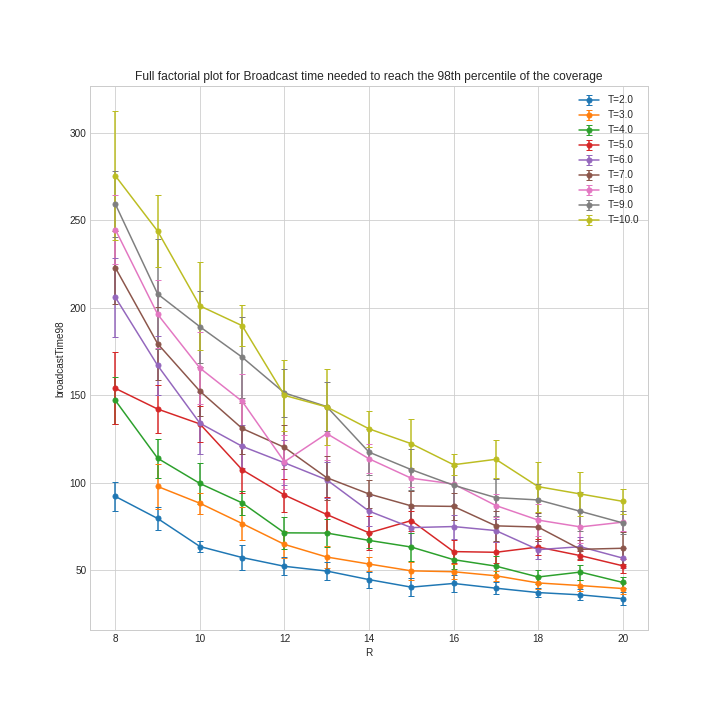
\includegraphics[width=0.8\textwidth]{img/hd/broadcasttime-R-ffplot}
	\caption{The broadcast time is lower with higher values of the broadcast
	radius and lower values of the size of the hear
	window (95\% confidence intervals)}\label{fig:hdtimeff}
\end{figure}

We can verify that the model derived with the \(2^{k}r\) analysis is valid. If we
compute, for example, the value for \(R\!=\!17m\) and \(T\!=\!10s\) using the
model we get the result shown in~\eqref{eq:hdtimepredictionexample} (values for
the two parameters are normalized between \(-1\) and \(1\)) which is near the
mean value obtained from the full factorial analysis (\(117.2s\)) and inside its
95\% confidence interval (\(106.7255\), \(127.6745\)).

\begin{equation}\label{eq:hdtimepredictionexample}
	t_B = e^{4.782874 - 0.462452 \cdot 0.4 + 0.240663 \cdot 1} =
	e^{4.8385562} \simeq 126.2869s
\end{equation}

If instead we want to optimize the \standout{energy efficiency}, we must reduce
the broadcast radius and the total number of messages sent. In file
\code{messages.ipynb} we have performed a factorial analysis with low values for
the broadcast radius. Other factors taken into considerations are the one we
have identified as relevant in \secref{subsec:hd2kr}, namely the maximum number
of copies and the size of the hear window. The configuration used is named
``HighDensityMessages''.

As we can see from \figref{fig:hdmessagesff}, we get that the maximum number of
copies hugely affects the total number of messages sent, as previously found by
the \(2^{k}r\) analysis. Surprisingly, the combination of the maximum number of
copies and the size of the hear window is very important to reduce the number of
messages sent (the lower lines in the plot are those with the higher values for
\(T\)). This contradicts what the \(2^{k}r\) analysis found before.

\begin{figure}[htb]
	\centering
	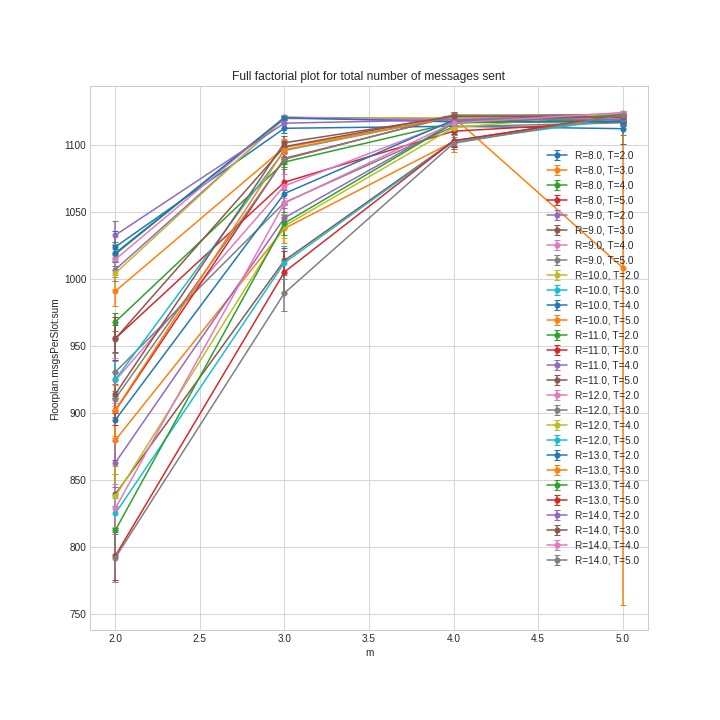
\includegraphics[width=0.8\textwidth]{img/hd/messages-m-ffplot}
	\caption{With low values of the maximum number of copies and higher
	values for the size of the hear window, we get a lower number of
	messages sent}\label{fig:hdmessagesff}
\end{figure}

So, in order to improve the energy efficiency, since we can not increase the
broadcast radius, we need to use a large \(T\) and a low \(m\). Increasing
\(T\) also increases the broadcast time, so a trade-off decision is needed in
this parameter. In order to account for both the indexes, one can increase the
value of \(R\) to reduce the broadcast radius and increase \(T\) maintaining a
low \(m\) in order to compensate for the increment of the energy consumption due
to the higher value of \(R\).

Regarding the \standout{total number of collisions}, we can reduce it by
reducing the broadcast radius and the maximum number of copies. Also helps
increasing the maximum relay delay. If the energy efficiency is the main
performance index that we want to optimize, the best way to reduce the total
number of collisions is certainly to reduce the broadcast radius. If instead we
want to optimize the broadcast time, we can reduce the total number of
collisions by reducing \(m\) and increasing \(\max(\delta)\). Factorial
analysis with the \(m\) and \(\max(\delta)\) parameters is available in
\code{collisions.ipynb}, using the configuration named
``HighDensityCollisions''. \figref{fig:hdcollisionsff} shows the results: the
plot is very well linear in the \(\max(\delta)\) parameter, suggesting that
increasing this factor even more should allow to have even a lower number of
collisions. \(m\!=\!2\) is a good setup for this parameter since it allows to
completely exploit the advantages of the \emph{trickle relaying} algorithm in
order to reduce the number of collisions and the number of messages sent.

\begin{figure}[hbt]
	\centering
	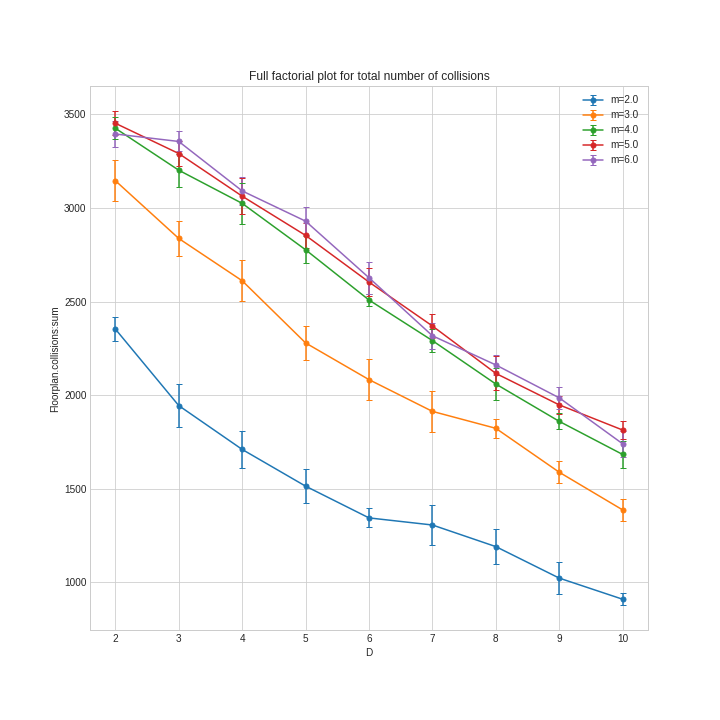
\includegraphics[width=0.8\textwidth]{img/hd/collisions-D-ffplot}
	\caption{The number of collisions is linearly dependent on the maximum
	relay delay. Also, trickle relaying can be exploited with low values of
	\(m\) in order to reduce the number of
	collisions}\label{fig:hdcollisionsff}
\end{figure}

\subsubsection{Conclusions}\label{subsubsec:hdconclusions}

\begin{itemize}
	\item The minimal configuration to get a nearly perfect coverage is with
		\(R\!=\!8m\), \(T\!=\!2s\), \(m\!=\!2\) and
		\(\max(\delta)\!=\!2s\). Higher values for these parameters does
		not break the coverage. For a more ``safe'' setup, \(R\) may be
		increased to \(9m\) or \(10m\).
	\item If a low total broadcast time is a main objective, increasing
		\(R\) is effective. Also reducing \(T\) allows for further
		improvement of the broadcast time.
	\item If instead a better energy efficiency is the main objective, \(R\)
		can not be increased and \(T\) should not be reduced. A
		trade-off decision between a low broadcast time and a good
		energy efficiency is needed.
	\item There is no reason to use large values for the maximum number of
		copies: \(m\!=\!2\) is a good set for this parameter and it
		leads to a lower number of collisions and a better energy
		efficiency without sacrificing the broadcast time. Trickle
		relaying is very effective in this job.
	\item \(\max(\delta)\) should be sufficiently high, in order to reduce
		the total number of collisions, but not too high, in order to
		avoid an increase in the broadcast time due to users waiting too
		much before relaying the message.
\end{itemize}
